\documentclass{article}
\linespread{1.3}
\usepackage[margin=50pt]{geometry}
\usepackage{amsmath, amsthm, amssymb, amsthm, tikz, fancyhdr, graphicx}
\pagestyle{fancy}
\renewcommand{\headrulewidth}{0pt}
\newcommand{\changefont}{\fontsize{15}{15}\selectfont}

\fancypagestyle{firstpageheader}
{
  \fancyhead[R]{\changefont Michael Huang \\ CFRM 420 \\ Homework 5}
}

\begin{document}

\thispagestyle{firstpageheader}

\section*{1.}
{\Large 

% \begin{verbatim}
%   Text enclosed inside \texttt{verbatim}
%   environment 
%   is printed directly 
%   and all \LaTeX{} commands are ignored.
% \end{verbatim}

% \framebox[1.1\width]{\textbf{answer}}

\subsection*{(a)}

See R file for the implementation: \\
\begin{verbatim}
  ORDINARY NONPARAMETRIC BOOTSTRAP


  Call:
  boot(data = data, statistic = cor.stat, R = 1)
  
  
  Bootstrap Statistics :
       original      bias    std. error
  t1* 0.6687307 0.001991947          NA
\end{verbatim}

\subsection*{(b)}

See R file for the implementation: \\
\begin{verbatim}
  ORDINARY NONPARAMETRIC BOOTSTRAP


  Call:
  boot(data = data, statistic = cor.stat, R = B)
  
  
  Bootstrap Statistics :
       original       bias    std. error
  t1* 0.6687307 6.870455e-05  0.01524621
\end{verbatim}

\subsection*{(c)}

We plot in R, and the distribution does seem to be approximately normal:
\begin{figure}[h!]
  \centering
  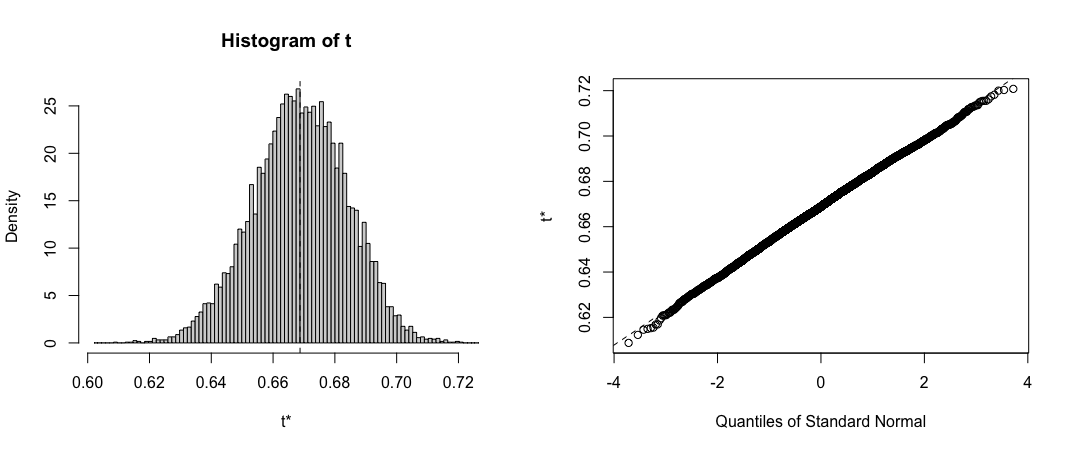
\includegraphics[width=500pt]{hw6_1c.png}
\end{figure}

\subsection*{(d)}

See R file for implementation: \\ 
\begin{verbatim}
  BOOTSTRAP CONFIDENCE INTERVAL CALCULATIONS
Based on 10000 bootstrap replicates

CALL : 
boot.ci(boot.out = bootcor, conf = 0.95, type = c("norm", "perc"))

Intervals : 
Level      Normal             Percentile     
95%   ( 0.6388,  0.6985 )   ( 0.6379,  0.6976 )  
Calculations and Intervals on Original Scale
\end{verbatim}

\subsection*{(e)}



}

\section*{2.}
{\Large

\subsection*{(a)}



\subsection*{(b)}



\subsection*{(c)}



}

\end{document}